\documentclass[11pt]{article}

\newif\ifBenchTikzExternalize
\BenchTikzExternalizefalse
\InputIfFileExists{bench-config.tex}{}{}

\newcommand{\benchtexttoken}{ALPHA}
\newcommand{\benchfiguretoken}{1.00}
\newcommand{\benchpreambletoken}{P0}

\usepackage{amsmath}
\usepackage{hyperref}
\usepackage{pgfplots}
\usepackage{tikz}
\usetikzlibrary{external}
\pgfplotsset{compat=1.18}

\ifBenchTikzExternalize
  \tikzexternalize[prefix=tikz-cache/]
\fi

\title{W4 TikZ Workload}
\author{FastXeBench}
\date{}

\begin{document}
\maketitle

\section{Purpose}
This workload stresses TikZ and pgfplots. The text token is \benchtexttoken, and the document keeps a citation path active via \cite{refalpha}.

\begin{figure}[p]
\centering
\tikzsetnextfilename{wave-a}
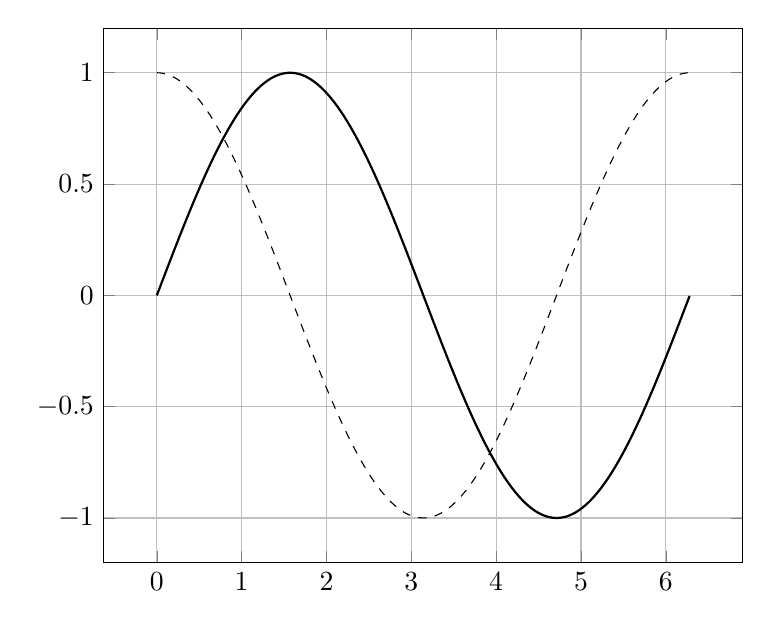
\begin{tikzpicture}
\begin{axis}[width=0.8\linewidth, grid=major, samples=160]
\addplot[thick, domain=0:6.28] {sin(deg(x)) * \benchfiguretoken};
\addplot[dashed, domain=0:6.28] {cos(deg(x))};
\end{axis}
\end{tikzpicture}
\caption{Smooth trigonometric curves.}
\label{fig:wave-a}
\end{figure}

\begin{figure}[p]
\centering
\tikzsetnextfilename{wave-b}
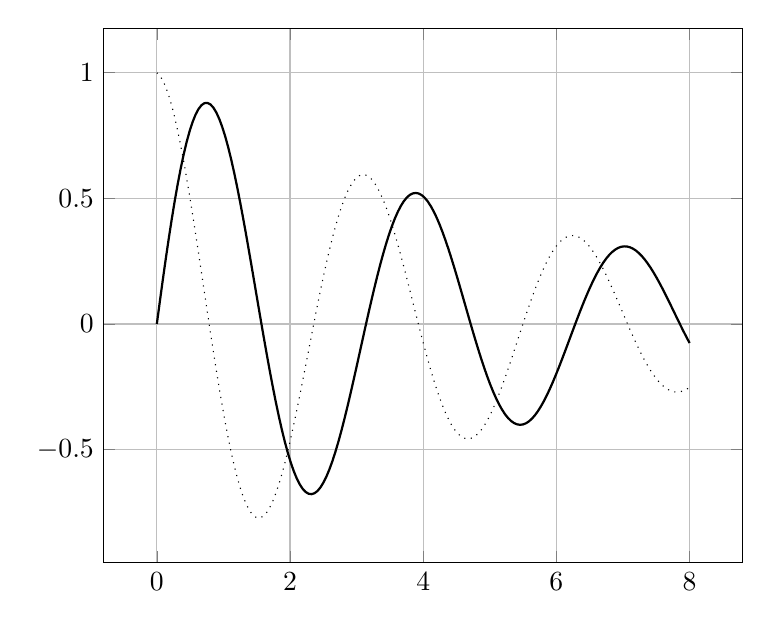
\begin{tikzpicture}
\begin{axis}[width=0.8\linewidth, grid=both, samples=180]
\addplot[thick, domain=0:8] {exp(-x/6) * sin(deg(2*x)) * \benchfiguretoken};
\addplot[dotted, domain=0:8] {exp(-x/6) * cos(deg(2*x))};
\end{axis}
\end{tikzpicture}
\caption{Damped oscillation.}
\label{fig:wave-b}
\end{figure}

\begin{figure}[p]
\centering
\tikzsetnextfilename{wave-c}
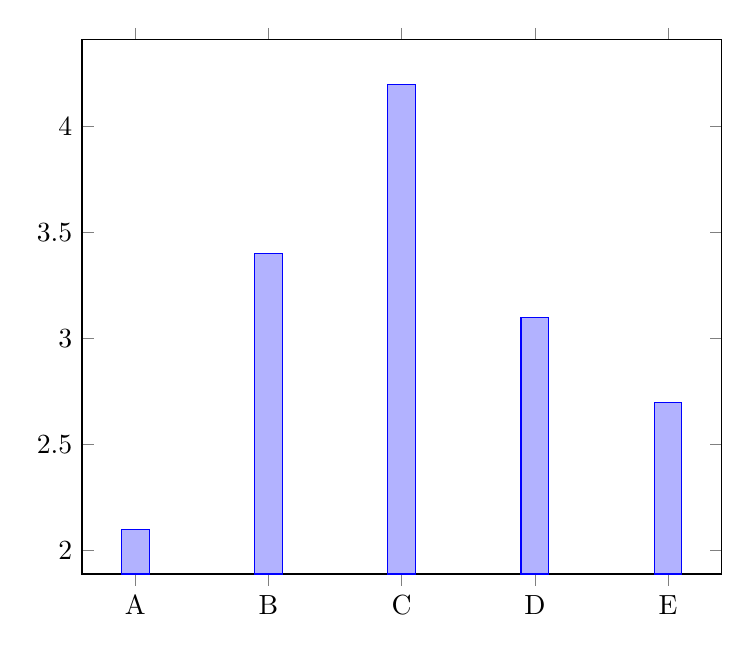
\begin{tikzpicture}
\pgfmathsetmacro{\finalbarheight}{2.7*\benchfiguretoken}
\begin{axis}[width=0.8\linewidth, ybar, symbolic x coords={A,B,C,D,E}, xtick=data]
\addplot coordinates {(A,2.1) (B,3.4) (C,4.2) (D,3.1) (E,\finalbarheight)};
\end{axis}
\end{tikzpicture}
\caption{A bar plot with a tunable final bar.}
\label{fig:wave-c}
\end{figure}

Figures~\ref{fig:wave-a}--\ref{fig:wave-c} are designed to benefit from externalization in steady-state runs.

\bibliographystyle{plain}
\bibliography{refs}

\end{document}
